\documentclass[../main.tex]{subfiles}
\begin{document}
\chapter{Requirements Engineering}
Per essere sicuri che una soluzione software risolva correttamente un problema del mondo reale dobbiamo prima comprenderlo completamente e definire: 
\begin{itemize}
	\item Quale problema sia da risolvere
	\item Il contesto da cui il problema parte
\end{itemize}
Definiamo come \textbf{mondo} la parte problematica del mondo reale, composto da componenti umani e componenti fisici.
Chiamiamo invece \textbf{macchina} (o sistema) ciò che deve essere installato per risolvere il problema, cioè software o soluzione hardware-software.
Il requirements engineering (RE) riguarda gli effetti della macchina sul mondo reale, le assunzioni e proprietà rilevanti del mondo.
\\ 
Il \textbf{system as-is} è il sistema allo stato attuale, precedente l'installazione della macchina.
Il \textbf{system to-be} è il sistema futuro, come sarà una volta installata la macchina.
\\
In una definizione preliminare di RE possiamo dire che è un insieme di attività volto a esplorare, valutare, documentare, consolidare, ripassare e adattare gli obiettivi, capacità, qualità, requisiti e assunzioni di un sistema software-intensive.
È basato sui problemi che sorgono nel sistema as-is e le opportunità portate dalle nuove tecnologie.
Le difficoltà principali del RE sono:
\begin{itemize}
	\item Scope ampio: diverse versioni del software (as-is, to-be, to-be-next) e ambienti ibridi (organizzazioni, leggi, politiche, device)
	\item Considerazioni multiple: funzionali, di qualità, di sviluppo.
	\item Livelli di astrazione
	\item Stakeholder multipli: con background diversi, interessi diversi e punti di vista contrastanti.
	\item Task intersecate durante il processo iterativo di elicitazione, valutazione, specifica e consolidazione.
\end{itemize}
Tre domande fondamentali che dobbiamo porci sono: perché installare un nuovo sistema? Quali servizi? Chi è responsabile per cosa?
\begin{itemize}
	\item \textbf{Perché?} Identificare, analizzare, rifinire gli obiettivi del sistema to-be per risolvere problematiche rilevate nel sistema as-is, allinearsi con gli obiettivi business e sfruttare nuove tecnologie.
	\\
	Le difficoltà principali sono:
	\begin{itemize}
		\item Acquisire conoscenze del dominio
		\item Valutare le varie alternative
		\item Identificare e risolvere conflitti tra obiettivi
	\end{itemize}
	\item \textbf{Cosa?} Identificare, definire i servizi funzionali del sistema to-be
	\begin{itemize}
		\item Soddisfare gli obiettivi identificati 
		\item In concomitanza con i requisiti di qualità: prestazioni, sicurezza\dots
		\item Basarsi su assunzioni realistiche dell'ambiente.
	\end{itemize}
	Le difficoltà principali sono:
	\begin{itemize}
		\item Identificare le feature corrette.
		\item Specificarle in maniera precisa in maniera che tutti possano capire.
		\item Assicurare la tracciabilità tra obiettivi.
	\end{itemize}
	\item \textbf{Chi?} Assegnare le responsabilità per gli obiettivi, servizi requisiti tra i componenti del sistema to-be.
	\begin{itemize}
		\item Basandosi sulle capacità e obiettivi del sistema.
		\item Definire il limite tra software e ambiente.
	\end{itemize}
	Le difficoltà principali sono:
	\begin{itemize}
		\item Valutare soluzioni alternative per decidere il giusto livello di automazione.
	\end{itemize}
\end{itemize}
\section{Tipi di requisiti}
Il modo in cui i requisiti vengono espressi possono essere divisi in \textbf{descrittivi} (modo indicativo) e \textbf{prescrittivo} (modo ottativo).
\\
\begin{tikzpicture}[
    node distance=2cm and 2.8cm,
    box/.style={
        draw,
        thick,
        rounded corners,
        fill=blue!10,
        align=center,
        minimum width=3.8cm,
        minimum height=1cm,
        font=\bfseries
    },
    arrowblue/.style={-Latex, thick, blue!70!black},
    arrowblack/.style={-Latex, thick, black}
]

% Nodes
\node[box] (env) {Environment};
\node[box, above=of env] (input) {Input Devices\\\normalsize(e.g.\ sensors)};
\node[box, above right=of env] (soft) {SoftwareToBe};
\node[box, right=of env] (output) {Output Devices\\\normalsize(e.g.\ actuators)};

% Arrows with side labels
\draw[arrowblack] (env) -- (input)
    node[midway, above left=2pt and 2pt] {\small M: monitored variables};

\draw[arrowblack] (input) -- (soft)
    node[midway, above =2pt and 2pt] {\small I:input data};

\draw[arrowblack] (soft) -- (output)
    node[midway, below right=2pt and 2pt] {\small O: output signals};

\draw[arrowblack] (output) -- (env)
    node[midway, below =2pt and 2pt] {\small C: controlled vars};

\end{tikzpicture}


\subsection{Requisiti di sistema}
Sistemi prescrittivi che si riferiscono a fenomeni dell'ambiente (non necessariamente condivisi).
Vengono soddisfatti dal sistema to-be, possibilmente integrato con altri componenti del sistema. Devono essere comprensibili da tutti gli stakeholder.
$SysReq\subseteq M\times C$ relazione tra ambiente monitorato e variabili controllate.
\subsection{Requisiti software}
Affermazioni prescrittive che si riferiscono a fenomeni condivisi tra ambiente e software. Vengono soddisfatti unicamente dal software, formulati nel vocabolario degli sviluppatori.
$SofReq\subseteq I\times O$ relazione tra input e output del software.
\subsection{Proprietà di dominio}
Affermazioni descrittive riguardanti i fenomeni del mondo (rimangono veri a prescindere del sistema to-be).
$Dom\subseteq M\times C$ leggi che non possono essere violate.
\subsection{Assunzioni}
Affermazioni che l'ambiente del software-to-be deve soddisfare. Formulate in termini di fenomeni di ambiente. Generalmente prescrittive (e.g. sensori e attuatori).
$Asm\subseteq M\times C \cup M\times I \cup C \times O$
\subsection{Definizioni}
Affermazioni che forniscono un preciso significato ai concetti di sistemi e termini ausiliari.
Non hanno valore di verità, non ha senso contestarle.
$sofReq=Map(SysReq, Asm, Dom)$
\\ \\
I requisiti si dividono ulteriormente in:
\begin{itemize}
	\item \textbf{Funzionali}: descrivono quali servizi il sistema deve fornire.
	\item \textbf{Non funzionali}: descrivono come il sistema deve essere (e.g. prestazioni, usabilità, affidabilità\dots).
\end{itemize}
\section{Qualità del software}
\begin{itemize}
    \item Completezza di obiettivi, requisiti e assunzioni
    \item Coerenza degli elementi del documento dei requisiti (RD)
    \item Adeguatezza di requisiti, assunzioni e proprietà del dominio
    \item Non ambiguità degli elementi del documento dei requisiti
    \item Misurabilità di requisiti e assunzioni
    \item Pertinenza di requisiti e assunzioni
    \item Fattibilità dei requisiti
    \item Comprensibilità degli elementi del documento dei requisiti
    \item Buona strutturazione del documento dei requisiti
    \item Modificabilità degli elementi del documento dei requisiti
    \item Tracciabilità degli elementi del documento dei requisiti
\end{itemize}
Errori nei documenti dei requisiti:
\begin{itemize}
    \item \textbf{Omissione:} caratteristica del mondo del problema non indicata in alcun elemento del documento dei requisiti (RD).\\
    \emph{Esempio:} nessun requisito riguardante lo stato delle porte del treno in caso di arresto di emergenza.
    
    \item \textbf{Contraddizione:} elementi del RD che descrivono una caratteristica del mondo del problema in modo incompatibile.\\
    \emph{Esempio:} ``Le porte devono essere sempre tenute chiuse tra le piattaforme'' e ``Le porte devono essere aperte in caso di arresto di emergenza.''
    
    \item \textbf{Inadeguatezza:} elemento del RD che non descrive in modo adeguato una caratteristica del mondo del problema.\\
    \emph{Esempio:} ``Se un libro non è stato restituito, il prestatore negligente deve essere avvisato che deve pagare una multa.''
    
    \item \textbf{Ambiguità:} elemento del RD che permette di interpretare una caratteristica del mondo del problema in modi diversi.\\
    \emph{Esempio:} ``Solo le persone che hanno partecipato ad almeno il 75\% delle riunioni possono essere premiate alla fine dell’anno.''
    
    \item \textbf{Non misurabilità:} elemento del RD che descrive una caratteristica del mondo del problema in modo tale da impedire il confronto tra opzioni o la verifica delle soluzioni.
\end{itemize}
Difetti nei documenti dei requisiti:
\begin{itemize}
    \item \textbf{Rumore (Noise):} elemento del RD che non fornisce alcuna informazione su caratteristiche del mondo del problema.\\
    \emph{Variante: ridondanza incontrollata.}\\
    \emph{Esempio:} ``Devono essere affissi cartelli di divieto di fumo sui finestrini del treno.''
    
    \item \textbf{Sovraspecificazione (Overspecification):} elemento del RD che descrive una caratteristica non presente nel mondo del problema, ma nella soluzione della macchina.\\
    \emph{Esempio:} ``Il metodo setAlarm deve essere invocato al ricevimento di un messaggio Alarm.''
    
    \item \textbf{Non fattibilità (Unfeasibility):} elemento del RD non implementabile entro i vincoli di budget o tempi.\\
    \emph{Esempio:} ``I pannelli a bordo del treno devono visualizzare tutti i voli in ritardo alla prossima fermata.''
    
    \item \textbf{Inintelleggibilità (Unintelligibility):} elemento del RD incomprensibile per chi deve utilizzarlo.\\
    \emph{Esempio:} ``Negli Stati Uniti, la nozione di NWO è diventata popolare dopo gli attacchi terroristici al WTC. Tuttavia, i funzionari della NATO e dell’OMC raramente fanno riferimento a un NWO nelle procedure relative al GATT, e si può dire che MVTO, la clausola MFN e gli SRO abbiano poco a che fare con un NOW.'' (da un comunicato stampa)
    
    \item \textbf{Scarsa strutturazione (Poor structuring):} elemento del RD non organizzato secondo alcuna regola sensata e visibile di strutturazione.\\
	\emph{Esempio:} ``Interconnessione dei controllo di accelerazione e problemi al tracking del treno``
    \item \textbf{Riferimento anticipato (Forward reference):} elemento del RD che utilizza caratteristiche del mondo del problema non ancora definite.\\
    \emph{Esempio:} uso multiplo del concetto di distanza di arresto nel caso peggiore prima che la sua definizione appaia alcune pagine dopo nel RD.
    
    \item \textbf{Rimpianto (Remorse):} elemento del RD che definisce una caratteristica del mondo del problema in modo tardivo o incidentale.\\
    \emph{Esempio:} dopo molteplici utilizzi del concetto non definito di distanza di arresto nel caso peggiore, l’ultimo uso è seguito direttamente da una definizione incidentale tra parentesi.
    
    \item \textbf{Scarsa modificabilità (Poor modifiability):} elementi del RD i cui cambiamenti devono essere propagati in tutto il documento.\\
    \emph{Esempio:} uso di valori numerici fissi per quantità soggette a variazioni.
    
    \item \textbf{Opacità (Opacity):} elemento del RD il cui razionale, autore o dipendenze sono invisibili.\\
    \emph{Esempio:} ``La velocità comandata del treno deve essere sempre almeno 7 mph superiore alla velocità fisica'' senza alcuna spiegazione del razionale di questa scelta.
\end{itemize}
\section{Processo di RE}
\begin{figure}[h]
    \centering
    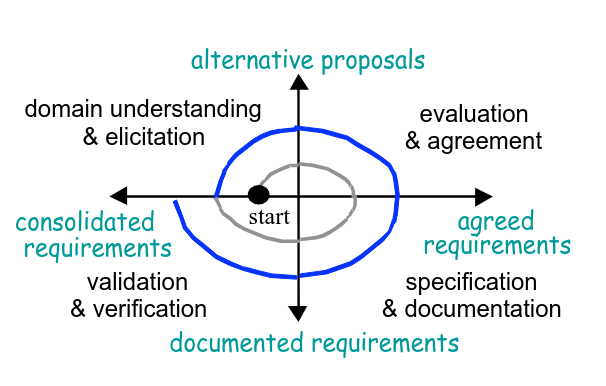
\includegraphics[width=0.7\textwidth]{pictures/RE.png}
\end{figure} \noindent
Per comprendere il dominio bisogna studiare il sistema as-is, identificare gli stakeholders, così da generare delle prime proposte di prototipi e il glossario dei termini.
\subsection{Elicitazione dei requisiti}
L'\textbf{elicitazione} dei requisiti esplora i problemi del mondo facendo ulteriori analisi del problema del sistema as-is, individuandone i sintomi, cause e conseguenze.
Vengono identificati:
\begin{itemize}
	\item Opportunità tecnologiche
	\item Obiettivi di miglioramento
	\item Requisiti tecnico-organizzativi del sistema to-be
	\item Soluzioni alternative per soddisfare gli obiettivi e assegnare le responsabilità
	\item Scenari ipotetici di interazione software-ambiente
	\item Requisiti software, assunzioni sull'ambiente
\end{itemize}
\subsection{Evaluazione e negoziazione dei requisiti}
Presa di decisioni basate sulla negoziazione. 
\begin{itemize}
	\item Identificazione e risoluzione di conflitti 
	\item Identificazione e risoluzione dei rischi del sistema proposto
	\item Confronto delle alternative tra obiettivi e rischi, selezione della soluzione preferita
	\item Priorità dei requisiti, per risolvere conflitti, considerare costi e supportare lo sviluppo incrementale.
\end{itemize}
Vengono prodotti le sezioni finali della proposta di prototipo che documentano gli obbiettivi concordati, i requisiti, le assunzioni e i ragionamenti che hanno portato ad essi.
\subsection{Specifiche e documentazione}
Definizione precisa di tutte le feature del sistema.
Obiettivi, proprietà di dominio rilevanti, requisiti, assunzioni, responsabilità.
Organizzare questi in una struttura coerente. Documentare in una forma comprensibile a tutti gli interessati. Viene prodotto il Requirements Document (RD).
\subsection{Consolidazione dei requisiti}
Attività per assicurare la qualità del RD. Vengono analizzate l'adeguatezza, la completezza, la mancanza di inconsistenze, vengono poi sistemati gli errori e i difetti. Viene prodotto un RD consolidato.

\end{document}